\documentclass{article}
\usepackage{lmodern}
\usepackage{upquote}
\usepackage{cite}
\usepackage{tikz}
\usepackage[hidelinks, pdfusetitle]{hyperref}

\usetikzlibrary{positioning}

\newcommand{\pytvversion}{0.5.6}

\title{PyTV: Python Templated Verilog}
\author{Wuqiong Zhao}

\begin{document}

\maketitle

\begin{abstract}
  PyTV (Python Templated Verilog)%
  \footnote{This is the documentation to PyTV version \texttt{\pytvversion{}}.
  Digital version of this document is available at \url{https://go.wqzhao.org/pytv-docs}.}
  is a Rust library and binary tool that extends Verilog with Python templating.
  Utilizing the flexibility of Python,
  PyTV allows users to write Verilog code with Python syntax and features
  including if statements, for loops, function definitions, etc.
  Moreover, PyTV supports instantiation of modules with complex parameters,
  and enables hierarchy extraction.
\end{abstract}

\tableofcontents

\section{Introduction}\label{sec:introduction}
% Templated languages
One method of auto generation of parameterized hardware relies on templated languages.
AHDW \cite{zhao2023automatic} is a language building upon Verilog with custom syntax for parameterized hardware.
% PyTV's advantage

Different from other domain-specific languages (DSLs) for hardware generation,
PyTV provides users with more control over the hardware architecture and implementation details.

% PyTV project information
PyTV is open-source at \url{https://github.com/autohdw/pytv}
and is distributed under the GPL-3.0 license.
The Rust crate is available at \url{https://crates.io/crates/pytv}.


\section{Installation}\label{sec:installation}
\subsection{Installation as a Rust Library}
Similar to other library crates, PyTV can be installed as a Rust library by adding the following line to the \texttt{Cargo.toml} file of your project:
\begin{verbatim}
[dependencies]
pytv = "0.5.6"
\end{verbatim}
The version number can be replaced with the desired version of PyTV.
The library can then be imported into your Rust code by adding the following line:
\begin{verbatim}
extern crate pytv;
\end{verbatim}

You can also install PyTV using the \texttt{cargo} command:
\begin{verbatim}
cargo install pytv
\end{verbatim}

\subsection{Installation as a Binary Tool}
PyTV can also be installed as a binary tool by running the following command:
\begin{verbatim}
cargo install pytv
\end{verbatim}

You can also build the binary tool from source by running the following command:
\begin{verbatim}
cargo build --release
\end{verbatim}

Note that the generation of Verilog files 


\section{Architecture}\label{sec:architecture}
The architecture (generation process) of PyTV is illustrated in Figure~\ref{fig:architecture}.

\begin{figure}[htbp]
  \centering
  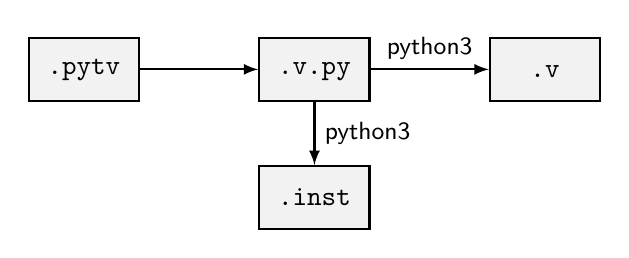
\begin{tikzpicture}[
    , thick
    , font = \sffamily
    , n/.style = {
      , draw
      , fill = gray!10
      , minimum width = 14mm
      , minimum height = 8mm
      , font = \ttfamily
      , text height = 1.3ex
    }
    , node distance = 8mm and 15mm
  ]
    \node (pytv) [n] {.pytv};
    \node (v-py) [n, right = of pytv] {.v.py};
    \node (v) [n, right = of v-py] {.v};
    \node (inst) [n, below = of v-py] {.inst};
    \draw [-latex] (pytv) -- (v-py);
    \draw [-latex] (v-py) -- (v) node [midway, above] {\small python3};
    \draw [-latex] (v-py) -- (inst) node [midway, right] {\small python3};
  \end{tikzpicture}
  \caption{Architecture of PyTV.}
  \label{fig:architecture}
\end{figure}


\section{Syntax Specifications}\label{sec:syntax}
\subsection{Basics: Python Line and Verilog Line}
As a general rule, a \textit{Python line} is a line of Python code,
and a \textit{Verilog line} is a line of Verilog code.
A minimal example is shown below:

\begin{verbatim}
//! a = 1 + 2;            #  Python inline
assign wire_`a` = wire_b; // Verilog line
/*!
b = a ** 2;               #  Python block
*/
\end{verbatim}

The syntax rule can be summarized as follows:
\begin{itemize}
  \item An \textit{inline Python line} starts with \texttt{//!}.
  \item A \textit{Python block} starts with \texttt{/*!} and ends with \texttt{*/}.
  \item Otherwise, it is a \textit{Verilog line}.
  In the Verilog line, contents in backticks (\verb|`|) are treated as Python variables,
  and are calculated inline.
\end{itemize}

Internally, a Python line will be copied to the generated \texttt{.v.py} file.
A Verilog line will be a \texttt{print} statement,
where contents in backticks (\verb|`|) are properly escaped and embedded in the format string.

\subsection{Indentation}
Because the generation framework is based on Python,
indentation is important.
The mixture of Python and Verilog code adds to the complexity.
Therefore, the following rules are enforced.

\textbf{Rule 1: same with Python.}
The number of spaces for Python indentation is a fixed number as required by Python.
It is recommended to use 4 spaces for Python indentation.

\textbf{Rule 2: no preceding spaces.}
For Python lines, no preceding spaces are allowed before the \texttt{//!}, \texttt{/*!}, or \texttt{*/}.
Otherwise they are not recognized as Python lines or blocks.

\textbf{Rule 3: first line decides for all.}

\textbf{Rule 4: proceeding lines follow.}

\textbf{Rule 5: ease with Verilog.}
The indentation of Verilog lines do not matter.
They will be printed as is.

\textbf{Rule 6: no tabs are allowed.}
Notably, tabs are strongly discouraged in PyTV, as it may lead to unexpected behavior due to indentation mismatch.
Always use spaces for indentation.

\subsection{Instantiation}
One important feature of PyTV is its capability to instantiate modules with complex parameters,
and to enable hierarchy extraction.


\section{Usage}\label{sec:usage}
\subsection{Rust Library Usage}

\textbf{Customization of the magic comment string.}

\subsection{Binary Tool Usage}


\section{Limitations}\label{sec:limitations}
\textbf{Important:}
PyTV is designed for research and prototyping purposes,
and is not intended for production use.


\section*{Further Readings}
\addcontentsline{toc}{section}{Further Readings}
Hardware generation using software programming languages is interesting to explore.
AHDW \cite{zhao2023automatic} is a previous attempt of implementation.
A high-level synthesis (HLS) library for Vitis HLS (in C++), FLAMES,
is proposed in \cite{zhao2024flexible}.

% auto generator of LEADS


\section*{Acknowledgments}
The author would like to thank members of the \href{https://github.com/autohdw}{\texttt{@autohdw}} team for
their support throughout the development of this project.
The author would also like to thank \textit{GitHub Copilot}
for providing code suggestions during the development of this project,
as well as the composition of this document.


\bibliographystyle{IEEEtran}
\phantomsection
\addcontentsline{toc}{section}{References}
\bgroup
\small
\bibliography{IEEEabrv, ref}
\egroup

\end{document}
